\chapter{Testing for Verification and Validation}
\label{ch:verification}

The PPP guideline distinguishes verification---solving the stated equations
correctly---from validation---representing the intended physical material.
The present work is verification-heavy because its principal contribution is
a software and numerical framework. Physical validation against experiments
remains limited and is stated as such.

\section{Phase 1: PyTorch--NGSolve proof of concept}

The first acceptance gate isolates the committee's central technical risk:
whether a PyTorch pICNN can supply a consistent hyperelastic stress and
tangent to an NGSolve equilibrium solve. Training labels come from the
analytical compressible neo-Hookean law, with \(\mu=1\) and \(\lambda=10\).
The following tests exercise the same constitutive and finite-element modules
used by the subsequent workflow. Each case records its aim, setup, command,
expected result, and observed result.

\subsection*{Test Case V1: Constitutive interface}
\paragraph{Aim.}
Verify the deformation-gradient input API and the shapes, data type, and
finiteness of the energy, first-Piola stress, and full tangent.

\paragraph{Setup.}
A float64 pICNN with a fixed random seed is evaluated at four admissible
deformation gradients near \(\Iten\). The test compares the public energy
interface with the invariant-feature interface.

\paragraph{How to run.}
\begin{lstlisting}[language=bash]
python -m tests.verify_model_interface
\end{lstlisting}

\paragraph{Expected result.}
The energy has shape \((4)\), stress has shape \((4,3,3)\), and the tangent
has shape \((4,3,3,3,3)\); all values are finite float64 quantities and both
stress interfaces agree.

\paragraph{Obtained result.}
All interface, shape, dtype, and finiteness assertions passed.

\subsection*{Test Case V2: Reference-state normalization}
\paragraph{Aim.}
Check that the normalized energy and its first derivative vanish at the
undeformed state.

\paragraph{Setup.}
The seeded float64 pICNN is evaluated at \(\F=\Iten\). Energy tolerance is
\(10^{-12}\); stress tolerance is scaled by the raw reference stress and
machine precision.

\paragraph{How to run.}
\begin{lstlisting}[language=bash]
python -m tests.verify_reference
\end{lstlisting}

\paragraph{Expected result.}
The affine reference correction must give \(\Psi(\Iten)=0\) and
\(\Pstress(\Iten)=\bm 0\) within the stated tolerances.

\paragraph{Obtained result.}
The recorded run gave zero energy error and zero maximum stress component;
the stress tolerance was \(2.220\times10^{-15}\). The test passed.

\subsection*{Test Case V2b: Neo-Hookean constitutive response}
\paragraph{Aim.}
Measure whether the trained pICNN reproduces the reference energy, stress,
and tangent before it is inserted into a finite-element solve.

\paragraph{Setup.}
The validated checkpoint is evaluated on 256 deterministic admissible
deformation gradients (seed 2026, maximum perturbation 0.2). The target is the
analytical compressible neo-Hookean material with \(\mu=1\) and
\(\lambda=10\). Relative \(L^2\) error limits are 10\% for energy, 10\% for
stress, and 25\% for the tangent.

\paragraph{How to run.}
\begin{lstlisting}[language=bash]
python -m tests.verify_neohooke_response --ckpt checkpoints/phase1_validated.pt
\end{lstlisting}

\paragraph{Expected result.}
All three relative errors must remain below their respective limits.

\paragraph{Obtained result.}
The recorded errors were 5.367\% for energy, 3.274\% for stress, and 3.865\%
for the tangent. All three limits were met. This verifies the reference
material response over the tested domain; it does not establish accuracy for
the later RVE-generated constitutive law.

\subsection*{Test Case V3: Automatic-differentiation tangent}
\paragraph{Aim.}
Verify the tangent \(\Aten=\partial\Pstress/\partial\F\) produced by
automatic differentiation and characterize the finite-difference diagnostic.

\paragraph{Setup.}
The exact PyTorch tangent is compared with central differences of stress for
four seeded deformation gradients. Perturbations range from \(10^{-2}\) to
\(10^{-8}\). Finite differences are used only for this check; the production
constitutive update uses automatic differentiation.

\paragraph{How to run.}
\begin{lstlisting}[language=bash]
python -m tests.verify_tangent
\end{lstlisting}

\paragraph{Expected result.}
The error should decrease as truncation error falls, then increase as
round-off dominates. A universal perturbation that reaches machine precision
is not assumed.

\paragraph{Obtained result.}
The archived run's relative errors were \(1.25\times10^{-5}\),
\(1.25\times10^{-9}\), \(1.69\times10^{-10}\), and
\(1.42\times10^{-8}\), respectively. The minimum occurred near
\(\epsilon=10^{-6}\), and the test passed its \(10^{-6}\) acceptance limit.
The non-monotone curve demonstrates the truncation--round-off trade-off; the
finite-difference values are not used to assemble the material tangent.

\subsection*{Test Case V4: Nonlinear finite-element equilibrium}
\paragraph{Aim.}
Verify that the integration-point transfer and consistent tangent produce
convergent NGSolve Newton iterations.

\paragraph{Setup.}
A unit cube is subjected to a 10\% displacement-controlled stretch in the
\(x\)-direction. The other faces are traction free. A seeded pICNN supplies
the material response through the custom integration-point bridge, with
first-order displacement elements. By default the seeded network is
untrained, isolating assembly and tangent consistency; an optional checkpoint
loads a trained Phase~1 network.

\paragraph{How to run.}
\begin{lstlisting}[language=bash]
python -m tests.verify_element
\end{lstlisting}

\paragraph{Expected result.}
The free residual must fall below \(10^{-8}\), with asymptotically quadratic
convergence once the iterates enter the local Newton regime.

\paragraph{Obtained result.}
The archived Phase~1 run converged in four Newton updates, reducing the free
residual from \(9.058\times10^{-1}\) to \(4.023\times10^{-11}\). The test
passed. The run is a nonlinear FE equilibrium check on a generated cube mesh;
it is not described as a one-element mesh test.

\begin{figure}[htbp]
\centering
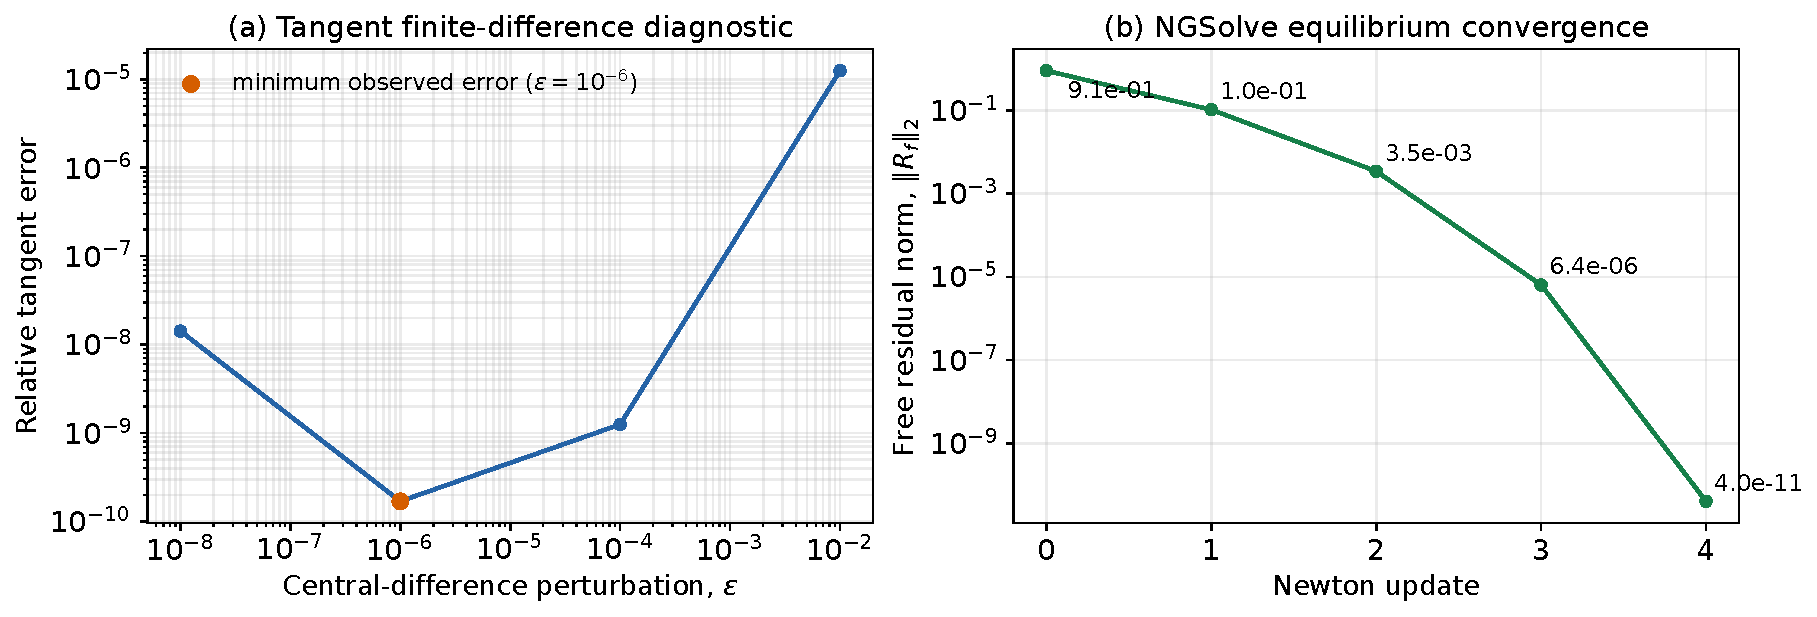
\includegraphics[width=\textwidth]{phase1_verification_diagnostics}
\caption{Archived Phase~1 verification diagnostics. (a) Relative error of a
central-difference stress tangent against the PyTorch automatic-differentiation
tangent for four perturbation sizes; finite differences are used only as a
check. (b) Free-residual history for the NGSolve nonlinear equilibrium
problem.}
\label{fig:phase1-diagnostics}
\end{figure}

\subsection*{Test Case V5: Affine patch}
\paragraph{Aim.}
Verify uniform deformation and stress, and zero free residual, on a
multi-element mesh using the same material transfer path.

\paragraph{Setup.}
A unit cube is assigned a mixed normal-strain and shear affine displacement
field corresponding to
\[
  \F_{\mathrm{target}}=
  \begin{bmatrix}
    1.08&0.05&0\\0&0.97&0.03\\0&0&1.02
  \end{bmatrix}.
\]
All boundary values are prescribed, leaving interior degrees of freedom for
the equilibrium check.

\paragraph{How to run.}
\begin{lstlisting}[language=bash]
python -m tests.verify_patch --ckpt checkpoints/phase1_validated.pt
\end{lstlisting}

\paragraph{Expected result.}
The sampled deformation gradient and stress must be uniform, and the
assembled residual on unconstrained degrees of freedom must vanish to
numerical precision.

\paragraph{Obtained result.}
On 206 elements and 2,884 material points, the maximum deformation-gradient
error was \(4.441\times10^{-16}\), relative stress variation was
\(4.774\times10^{-15}\), and free residual norm was
\(2.083\times10^{-16}\). The patch test passed.

\subsection*{Test Case V6: Matched analytical and neural FE problems}
\paragraph{Aim.}
Compare the nonlinear FE fields and reactions obtained with the neural
material against the same problem solved with the analytical neo-Hookean law.

\paragraph{Setup.}
Both material models solve the same unit-cube problem under 10\% prescribed
stretch in the \(x\)-direction, with traction-free lateral faces and
first-order displacement elements. Acceptance limits are 15\% for free
displacement, deformation gradient, and reaction-vector relative errors.

\paragraph{How to run.}
\begin{lstlisting}[language=bash]
python -m tests.verify_fe_comparison --ckpt checkpoints/phase1_validated.pt
\end{lstlisting}

\paragraph{Expected result.}
Both nonlinear solves must converge, and the three comparison errors must
fall below 15\%.

\paragraph{Obtained result.}
Both solves converged. Relative errors were 1.376\% for free displacement,
0.3504\% for the deformation gradient, and 13.60\% for the reaction vector.
All acceptance limits were met. The reaction error is close to its limit and
is evidence for the Phase~1 interface proof, not production accuracy.

\begin{figure}[htbp]
\centering
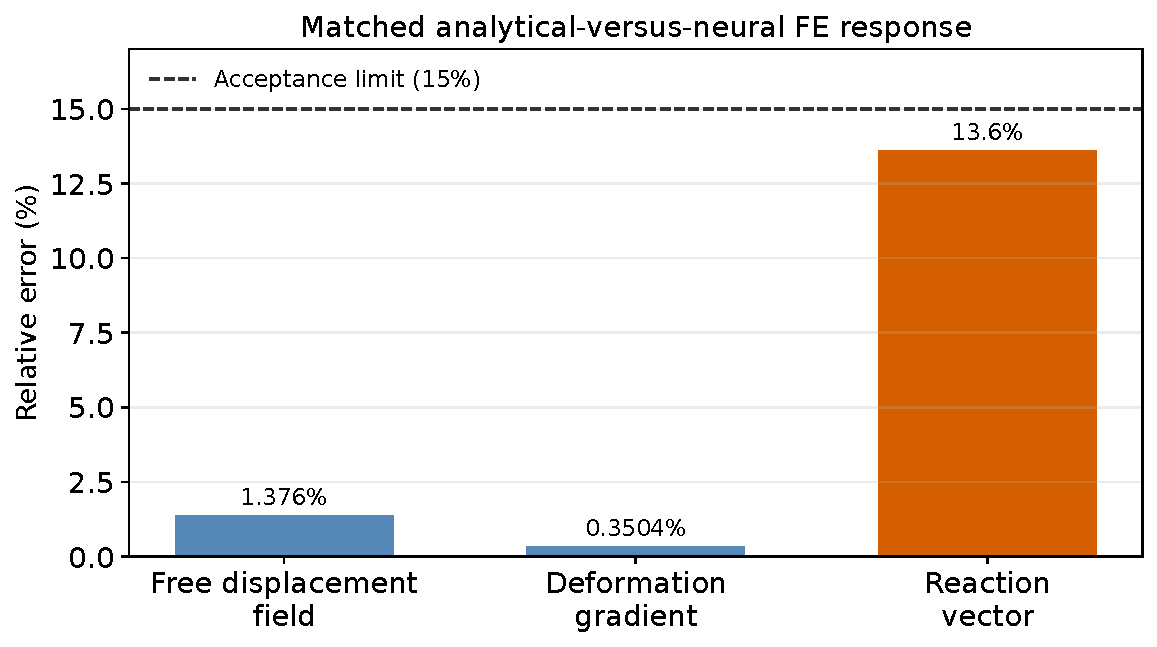
\includegraphics[width=0.82\textwidth]{phase1_matched_fe_errors}
\caption{Relative differences between the matched analytical
neo-Hookean and neural-material FE solutions. The dashed line is the
15\% acceptance limit. The reaction-vector error is the closest quantity
to that limit.}
\label{fig:phase1-fe-errors}
\end{figure}

\section{Verification matrix}

\begin{longtable}{@{}p{0.10\textwidth}p{0.30\textwidth}p{0.24\textwidth}p{0.22\textwidth}@{}}
\caption{Verification gates and their numerical evidence.}
\label{tab:verification-matrix}\\
\toprule
ID & Aim & Expected result & Status/evidence\\
\midrule
\endfirsthead
\toprule
ID & Aim & Expected result & Status/evidence\\
\midrule
\endhead
V1 & Constitutive API & Correct tensor shapes and interfaces & Passed\\
V2 & Reference normalization & \(\Psi(\Iten)=0,\ \Pstress(\Iten)=0\) & Passed\\
V2b & Analytical material response & Agreement with neo-Hookean reference & Passed\\
V3 & AD tangent & V-shaped finite-difference diagnostic & Passed\\
V4 & Nonlinear FE equilibrium & Residual below \(10^{-8}\) & Passed\\
V5 & Affine patch & Uniform \(\F\), zero free residual & Passed\\
V6 & Matched FE problems & Neural/analytical field comparison & Passed\\
P2-V1 & Periodic space & Opposite-face trace equality & \(5.516\times10^{-16}\)\\
P2-V2 & Rigid kinematics & Six modes, proper finite rotation & Passed\\
P2-V3 & Mixed patch & Exact affine \(F,J,p\) at \(\kappa/\mu=10^4\) & Passed\\
P2-V4 & Coupled RVE & Periodic and rigid equilibrium & Passed\\
P2-V5 & Hill--Mandel & Equal macro/micro virtual work & \(1.085\times10^{-13}\)\\
P2-V6 & Condensed tangent & Symmetry and second-order Taylor remainder & Passed\\
P2-V7 & Free rotation & Zero particle moment & \(1.436\times10^{-15}\)\\
P2-V8 & Translation gauge & Physical fields invariant to constant shift & Passed\\
P2-V9 & Rotational tangent & Condensed force--moment sensitivities & Passed\\
P2-V10 & Dataset contract & Deterministic splits and serialization & Passed\\
S-V1 & Surrogate derivatives & Energy gradient, tangent direction, objectivity
and symmetry & Passed on independent states\\
M-V1 & First-order macro solve & Reach 5\% stretch with finite,
orientation-preserving states & Passed at three meshes\\
M-V2 & Second-order macro solve & Reach 5\% stretch & Not passed\\
\bottomrule
\end{longtable}

\section{Phase 2: homogenization and surrogate tests}

\subsection*{Test Case P2-V5: Hill--Mandel macrohomogeneity}

\paragraph{Aim.}
Verify that the discretely homogenized first-Piola stress is work-conjugate to
the imposed macroscopic deformation gradient.

\paragraph{Setup.}
A periodic unit-cell matrix with a centered rigid spherical particle is
subjected to finite hydrostatic loading. The matrix uses the mixed
\(P_2/P_1\) formulation with \(\kappa/\mu=10^4\). Particle translation follows
the mapped center, and the fluctuation satisfies periodic constraints.

\paragraph{How to run.}
\begin{lstlisting}[language=bash]
python -m tests.verify_hill_mandel
\end{lstlisting}

\paragraph{Expected result.}
For every admissible virtual rate, the macro and micro powers in
\cref{eq:hill-mandel} must agree. A constant-stress recovery test must also
confirm sign, index ordering, and total-volume normalization.

\paragraph{Obtained result.}
The reaction-based formulation produced a relative mismatch of
\(1.085\times10^{-13}\), an alternative virtual-field error of
\(5.656\times10^{-13}\), and a constant-stress recovery error of
\(3.553\times10^{-14}\). Raw boundary-stress recovery remained at
\(3.859\times10^{-6}\) and is retained only as a diagnostic.

\section{Independent surrogate constitutive checks}

\paragraph{Aim.}
Check that the learned scalar energy, stress, and tangent remain mutually
consistent and objective on deformation states not used to train the evaluated
Phase~6 checkpoint.

\paragraph{Setup and how to run.}
The Phase~7 independent dataset uses seed 4103, three volume fractions, and
targeted compression and expansion states. The command is:
\begin{lstlisting}[language=bash]
python -m benchmarks.rve_surrogate_constitutive_checks \
  --dataset <phase7.npz> --manifest <phase7.manifest.json> \
  --checkpoint <phase6.pt> --training-dataset <phase6.npz> \
  --report constitutive_checks.json \
  --states-per-det-bin 2 --fd-step 1.0e-5 --torch-threads 4
\end{lstlisting}

\paragraph{Expected and obtained result.}
All six errors must remain below their stored thresholds. Across 12
deformation states and 36 volume-fraction records, the largest energy-gradient
and tangent-direction errors were \(1.959\times10^{-7}\) and
\(7.809\times10^{-9}\). Maximum objectivity errors were
\(6.537\times10^{-13}\) for energy, \(9.921\times10^{-13}\) for stress, and
\(4.108\times10^{-15}\) for tangent; tangent symmetry error was
\(1.134\times10^{-15}\). The report status is \texttt{pass}. These checks
verify constitutive implementation but do not establish physical accuracy.

\section{Validation status}

Numerical surrogate assessment uses grouped holdouts and independent RVE
campaigns. The selected shear-adapted checkpoint was evaluated on 12 new
direct-RVE simple-shear cases spanning three volume fractions and four
amplitudes, with a microstructure seed distinct from the adaptation data. It
reduced mean relative \(P_{01}\) error from 58.8\% to 40.1\% and stress
Frobenius relative RMSE from 64.3\% to 46.6\%. These errors remain substantial,
and the test covers only one new microstructure realization. The selected
checkpoint also completed a matched first-order macro-FE run to 5\% stretch
with positive sampled Jacobians. A second-order mesh refinement completed at
0.5\% stretch, but second-order 5\% loading and broader quadrature convergence
remain unresolved. No experimental PDMS--glass validation is available, and
none is claimed.
